\chapter{Implementation}
\label{ch:implementation}

This chapter describes the implementation of the system. The description follows the layering established in Chapter~\ref{ch:design}: the data layer, the attack-graph layer, the simulation layer, the optimization layer, and the UI layer. The implementation is small enough to be discussed end-to-end, and the most important parts are illustrated with code excerpts.

\section{Attack-Graph Layer}

The attack-graph layer is implemented as a small set of Elixir modules. The central data structure is a directed graph whose nodes are \mintinline{elixir}|%NetworkDefense.AttackGraph.Node{}| records and whose edges are \mintinline{elixir}|%NetworkDefense.AttackGraph.Edge{}| records. The graph is built in two passes: a structural pass that follows the network reachability relation, and an enrichment pass that adds edges for each applicable CVE. Source Code~\ref{src:impl:graph} shows the entry point of the graph builder.

\begin{code}
	\begin{minted}{elixir}
defmodule NetworkDefense.AttackGraph do
  alias NetworkDefense.AttackGraph.{Node, Edge}

  def build(topology, cve_feed) do
    base_nodes = topology.hosts
                 |> Enum.flat_map(&host_service_nodes/1)
    base_edges = topology.reachability
                 |> Enum.flat_map(&reachability_edges/1)
    enriched_edges = base_edges
                     |> Enum.flat_map(&cve_edges(&1, cve_feed))
    %{nodes: base_nodes, edges: base_edges ++ enriched_edges}
  end
end
	\end{minted}
	\caption{Entry point of the attack-graph builder.}
	\label{src:impl:graph}
\end{code}

The choice of a two-pass construction is deliberate: it keeps the structural and enrichment concerns in separate functions, and it makes it easy to add a third pass later (e.g., for transitive-vulnerability inference) without changing the upstream passes.

\section{Simulation Layer}

The simulation layer is implemented as a single \mintinline{elixir}|NetworkDefense.Simulator| module. The module exposes a \mintinline{elixir}|run/3| function that takes a graph, an entry point, and a number of iterations, and returns a blast-radius map. The pipeline is illustrated in Figure~\ref{fig:impl:pipeline}.

\begin{figure}[hbt!]
	\centering
	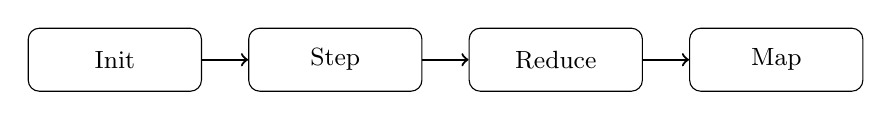
\begin{tikzpicture}[
			every node/.style={align=center, draw, rectangle, rounded corners, minimum width=2.2cm, minimum height=0.8cm, font=\small},
			arrow/.style={->, thick},
		]
		\node (p1) at (0, 0) {Init};
		\node (p2) at (2.8, 0) {Step};
		\node (p3) at (5.6, 0) {Reduce};
		\node (p4) at (8.4, 0) {Map};

		\draw[arrow] (p1) -- (p2);
		\draw[arrow] (p2) -- (p3);
		\draw[arrow] (p3) -- (p4);
	\end{tikzpicture}
	\caption{The four stages of the simulator pipeline.}
	\label{fig:impl:pipeline}
\end{figure}

The simulator step itself is shown in Source Code~\ref{src:impl:step}. It is a small recursive function over the attack graph; the recursion is bounded by the iteration budget and the depth of the graph.

\begin{code}
	\begin{minted}{elixir}
defp step(graph, current, reached, depth) do
  outgoing = outgoing_edges(graph, current)

  case Enum.random(outgoing) do
    nil ->
      reached

    edge ->
      if :rand.uniform() < edge.probability and depth > 0 do
        step(graph, edge.target, MapSet.put(reached, edge.target), depth - 1)
      else
        reached
      end
  end
end
	\end{minted}
	\caption{One step of the Monte Carlo simulator.}
	\label{src:impl:step}
\end{code}

\section{Optimization Layer}

The optimization layer is implemented in three sibling modules, one per strategy:

\begin{itemize}
	\item \mintinline{elixir}|NetworkDefense.Optimizer.MinCut|
	\item \mintinline{elixir}|NetworkDefense.Optimizer.Greedy|
	\item \mintinline{elixir}|NetworkDefense.Optimizer.Hybrid|
\end{itemize}

\noindent Each module exposes a \mintinline{elixir}|recommend/2| function with the same signature, so they are interchangeable at the call site.

The min-cut strategy is implemented in terms of a small Stoer--Wagner implementation; the greedy strategy is implemented in terms of a sort over the marginal blast-radius reduction of each vulnerability. The hybrid strategy alternates the two and uses the better of the two at each step.

A small auxiliary routine, \mintinline{elixir}|marginal_reduction(graph, blast_map, action)|, encapsulates the cost of evaluating a single candidate action. Listing it here is not necessary for the narrative; what matters is that the call site in the optimizer loop is a single line.

\section{UI Layer}

The UI layer is a Phoenix LiveView application. The main page renders the current blast-radius map as a heat map, lists the top recommended defensive actions, and shows a side-by-side comparison of the current and post-defense blast-radius maps. The user can step through the recommended actions one at a time, and the visualization updates in real time as each action is applied.

The choice of LiveView is driven by the need for low-latency interaction: the user typically wants to see the effect of each candidate action immediately, and a full HTTP round-trip per action would be too slow.
